% Institutional profiles under a common prudential framework. ICA CCR 2026, Valencia.
% Ten-minute paper presentation (Session 3, Public policy and institutional support for
% cooperatives, 4 November 2026; programme title "Credit Cooperatives vs. Banks Under Identical
% Basel-Style Regulation in Brazil", paper 294).
% Compile with pdfLaTeX twice (MiKTeX locally, installed 2026-10-28, or Overleaf via slides_overleaf.zip).
% Speaker notes: uncomment ONE of the two lines below.
% \setbeameroption{show notes on second screen=right}
% \setbeameroption{show only notes}
% Figures: figures/ (copied from ../figures by slides/make_slide_figures.py, which also draws the
% slide-only figures from tables/*.txt). Tables: tables/ (copies of ../tables/*.tex). Numbers typed
% in the slides come from tables/t1, t2, t3, t5, t7, t8, t13 and the manuscript; the source is
% named in a comment beside each.
\documentclass[aspectratio=169,10pt]{beamer}
\usepackage[T1]{fontenc}
\usepackage[utf8]{inputenc}
\usepackage{lmodern}
\usepackage{booktabs,graphicx,amsmath,amssymb,array,threeparttable}
\usepackage{tikz}
\usetikzlibrary{positioning,arrows.meta,calc}
\graphicspath{{figures/}}


% ---------------------------------------------------------------- theme: default Beamer theme, Computer Modern, Sistema OCB logo
\usetheme{default}
\setbeamertemplate{navigation symbols}{}
\setbeamertemplate{note page}{\small\insertnote}
\definecolor{deep}{rgb}{0.2,0.2,0.7}% Beamer's structure blue
\definecolor{muted}{gray}{0.35}
\definecolor{paper}{gray}{0.92}
\colorlet{ink}{black}
\definecolor{coop}{HTML}{2A78D6}% palette of the paper's figures, used in the design diagram
\definecolor{bank}{HTML}{EB6834}
\setbeamertemplate{footline}{\leavevmode\hbox to \paperwidth{\hspace{0.35cm}\raisebox{0.1cm}{
\includegraphics[height=0.42cm]{logo_sistema_ocb}}\hfill
  {\tiny\color{muted}\insertshorttitle\quad ICA CCR 2026\quad\insertframenumber}\hspace{0.35cm}}\vspace{0.1cm}}
\titlegraphic{
\includegraphics[height=0.9cm]{logo_sistema_ocb}}

\newcommand{\bignum}[2]{{\centering{\color{deep}\fontsize{22}{24}\selectfont\bfseries #1}\par\vspace{2pt}{\scriptsize\color{muted} #2}\par}}
\newcommand{\card}[3]{\begin{block}{#2}\scriptsize #3\end{block}}% #1 (width) kept for compatibility; the block fills its column
\newcommand{\divider}[4]{\begin{frame}[plain]\centering\vfill{\color{deep}\large #1}\par\vspace{6pt}{\color{deep}\fontsize{24}{28}\selectfont\bfseries #2}\par
  \vspace{10pt}{\large #3}\vfill\note{#4}\end{frame}}
\tikzset{box/.style={fill=paper,inner sep=5pt,align=center,font=\footnotesize,text width=#1},
  arr/.style={-{Stealth[length=5pt]},thick,color=muted}}

\title[Cooperatives and banks under a common prudential framework]{Institutional profiles under a common prudential framework}
\subtitle{Evidence from Brazilian credit cooperatives and banks}
\author{Arthur Gomes Nery \and Thiago de Oliveira Victorino \and Rodrigo Lima Rangel}
\institute{Organization of Brazilian Cooperatives (OCB System)}
\date{ICA CCR Research Conference, Valencia, 4 November 2026\\[2pt]{\small Paper 294, Session 3: Public policy and institutional support for cooperatives}}

\begin{document}

% ================================================================ title
\begin{frame}[plain]
\titlepage
\note{Ten minutes. The question: once a credit cooperative computes capital and risk under the same Basel-style rules as a commercial bank, does the cooperative form still leave a mark on the balance sheet? Brazil gives us the setting to ask it on the full population of institutions under the full methodology.}
\end{frame}

\begin{frame}{One rulebook for two forms}
\centerline{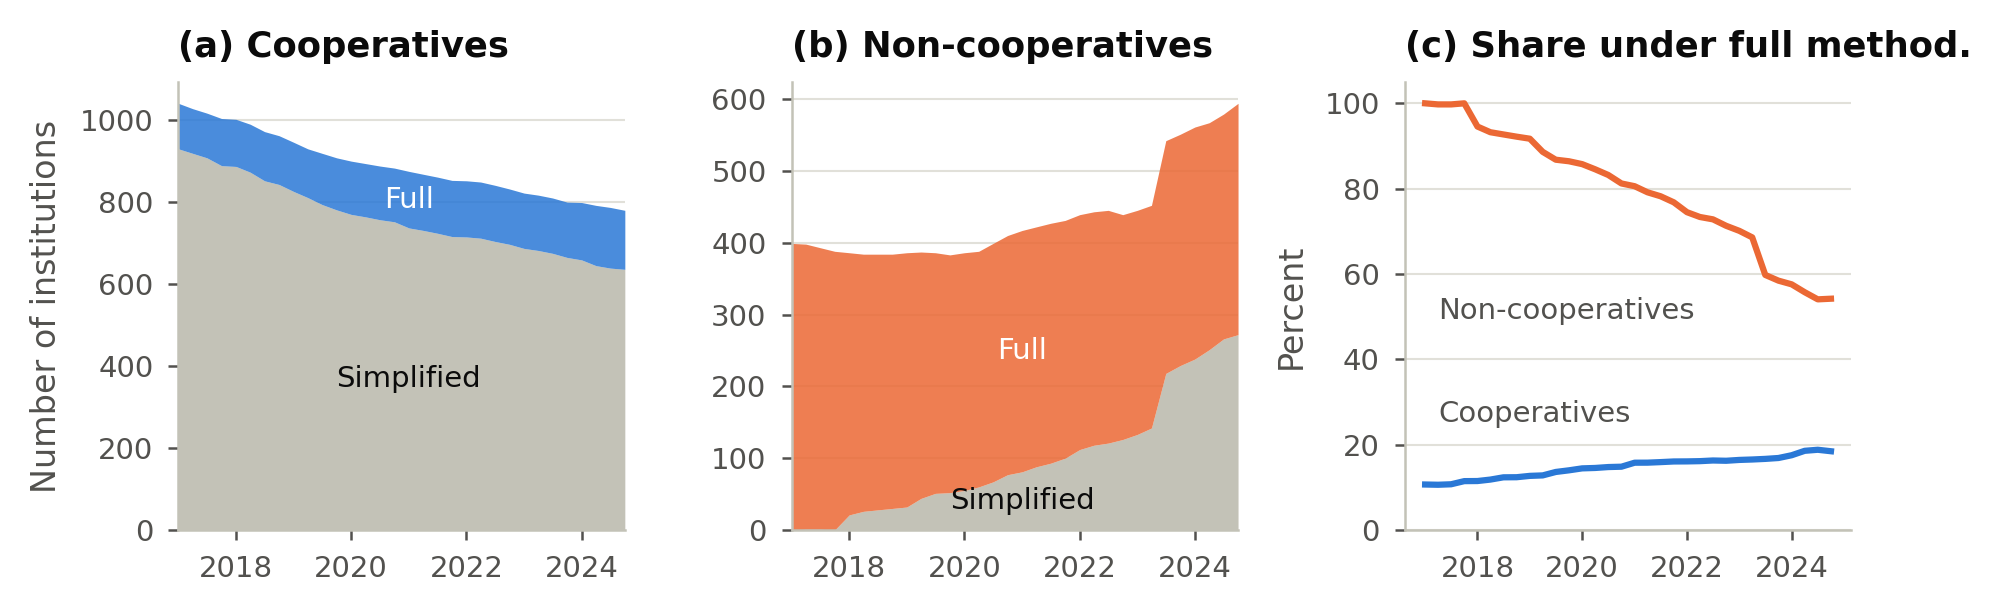
\includegraphics[width=0.8\linewidth]{fig5_regulatory}}
\vspace{0.1cm}
\begin{columns}[T]
\column{0.32\textwidth}\card{3.9cm}{The threshold}{Five segments. S1 to S4 apply the full Basel methodology; small institutions may opt for a simplified method (S5). Banks are excluded from S5 at any size.}
\column{0.32\textwidth}\card{3.9cm}{The same rules}{A cooperative above the threshold, or declining the simplified option, computes capital, risk weights and provisions as a commercial bank does.}
\column{0.32\textwidth}\card{3.9cm}{One rule apart}{Cooperative acts, the operations with members, are untaxed; banks pay income tax and the social contribution. Profitability is measured before and after tax.}
\end{columns}
\note{One minute. About 140 cooperatives are under the full methodology, a rising share. The prudential rules are held fixed by construction. The fiscal rules are not, and that difference becomes one of the results.}
\end{frame}

\begin{frame}{Data and design}
\begin{columns}[T]
\column{0.5\textwidth}
\vspace{0.1cm}
\card{6.3cm}{Panel}{IF.data, the Central Bank of Brazil's public repository. Every cooperative and bank under the full methodology, 2017Q1 to 2024Q4: 130 singular credit cooperatives, 144 banks, 7,234 institution-quarters. Central cooperatives excluded.}
\card{6.3cm}{Inference}{Standard errors clustered by institution; every coefficient confirmed by a wild cluster bootstrap. Conditional medians and quantile regressions beside the means. Cooperative status is time-invariant, so the estimates are conditional correlations.}
\column{0.48\textwidth}
\begin{center}
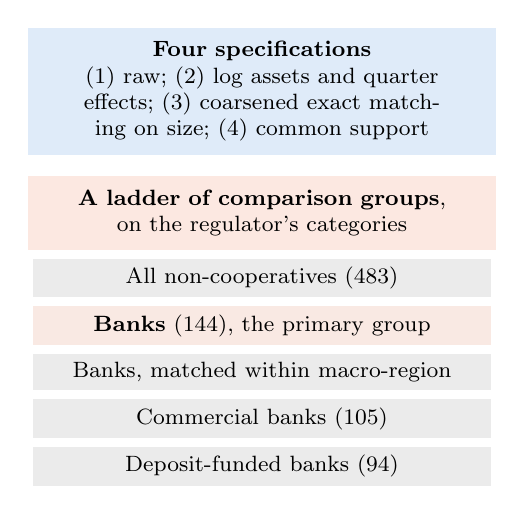
\begin{tikzpicture}[node distance=0.1cm and 0.5cm]
\node[box=5.6cm,fill=coop!15] (s) {\textbf{Four specifications}\\(1) raw; (2) log assets and quarter effects; (3) coarsened exact matching on size; (4) common support};
\node[box=5.6cm,below=0.25cm of s,fill=bank!15] (l) {\textbf{A ladder of comparison groups}, on the regulator's categories};
\node[box=5.6cm,inner sep=3pt,below=of l] (r1) {All non-cooperatives (483)};
\node[box=5.6cm,inner sep=3pt,below=of r1,fill=paper!60!bank!30] (r2) {\textbf{Banks} (144), the primary group};
\node[box=5.6cm,inner sep=3pt,below=of r2] (r3) {Banks, matched within macro-region};
\node[box=5.6cm,inner sep=3pt,below=of r3] (r4) {Commercial banks (105)};
\node[box=5.6cm,inner sep=3pt,below=of r4] (r5) {Deposit-funded banks (94)};
\end{tikzpicture}
\end{center}
\end{columns}
\note{One minute. Eleven outcomes: capital ratio, leverage, return on assets after and before tax, intermediation margin, cost-to-income, credit share, provisioning, funding, and return volatility and z-score at the institution level. Two things to retain. First, four specifications and a matched sample, so that we compare cooperatives with banks of the same size. Second, the comparison group is a reported parameter: a ladder from every non-cooperative institution down to banks that take deposits in every quarter. Which rung you choose turns out to decide several results.}
\end{frame}

\begin{frame}{The profile in one picture}
\begin{columns}[T]
\column{0.7\textwidth}
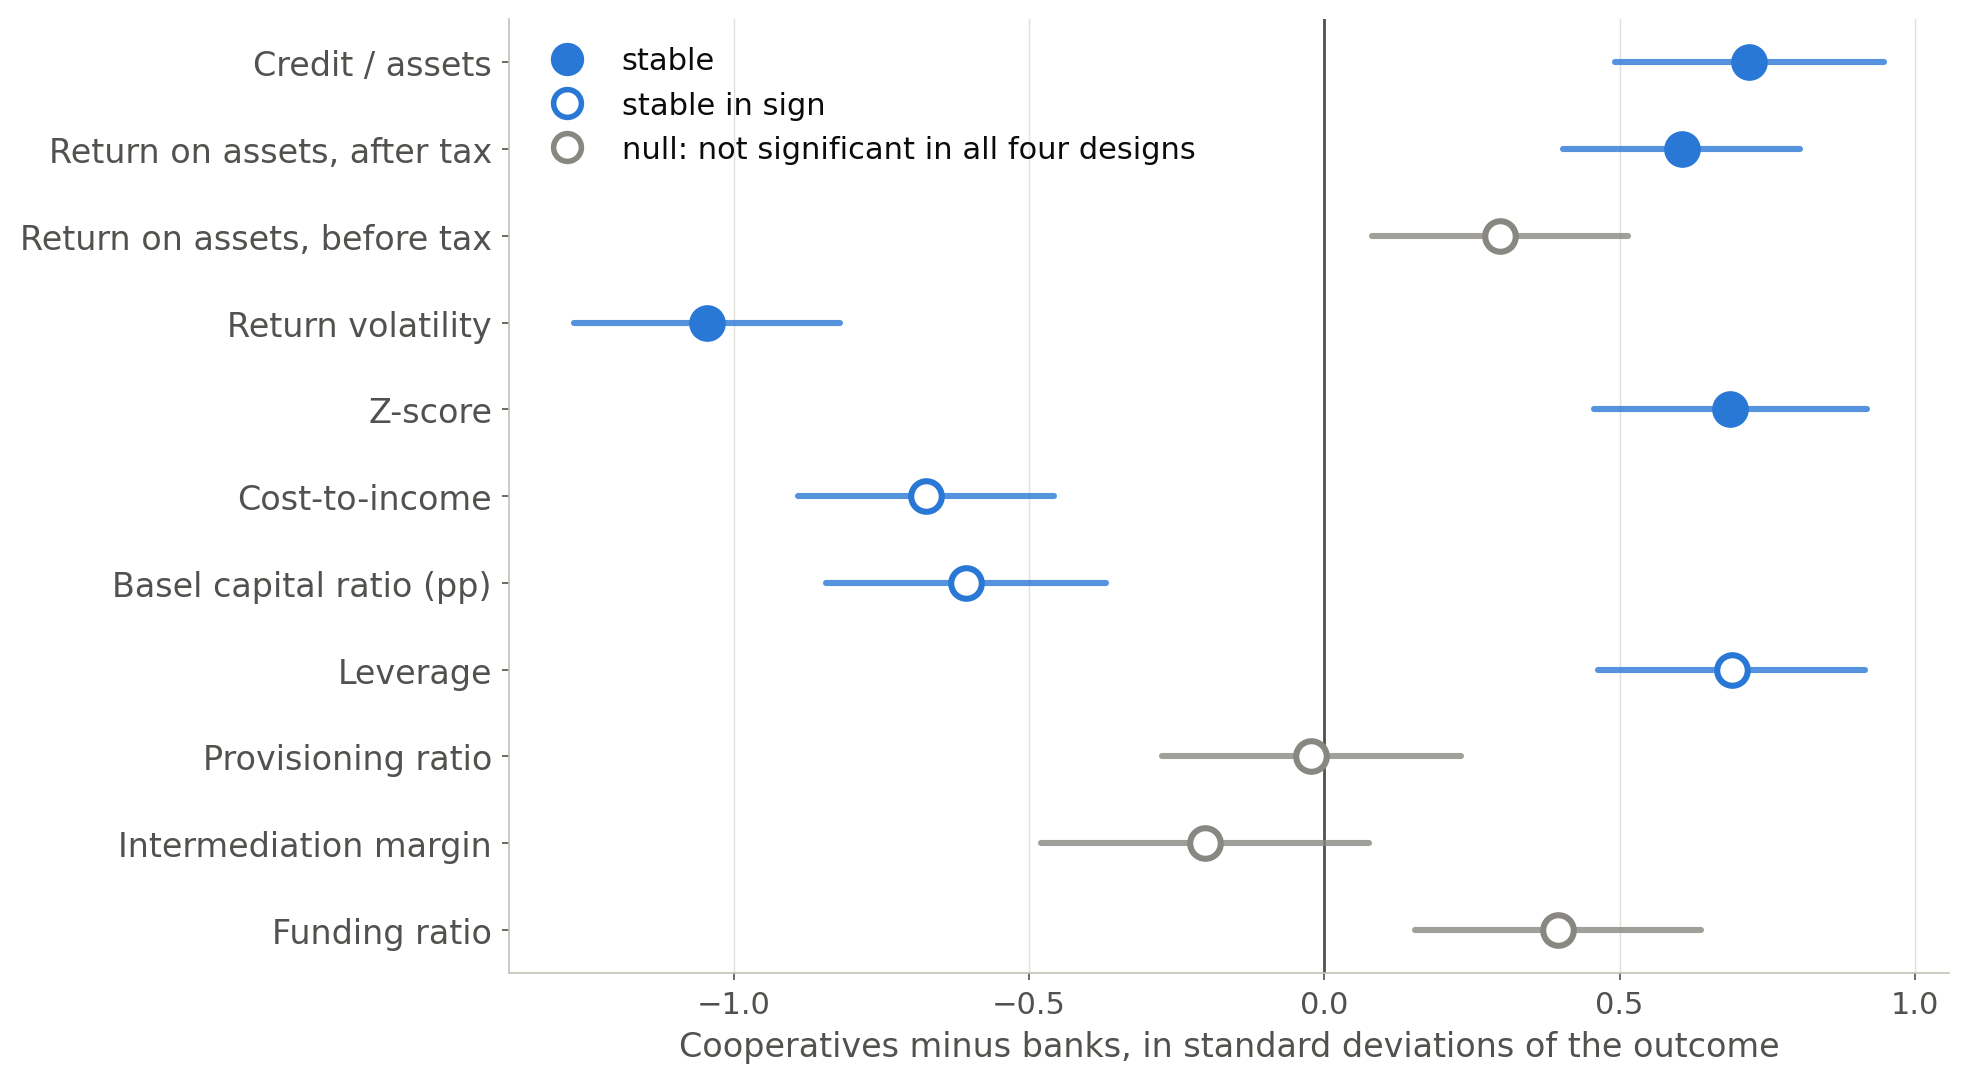
\includegraphics[width=\linewidth]{profile}
\column{0.28\textwidth}
\vspace{0.15cm}
\card{3.5cm}{Reading}{Cooperatives minus banks of comparable size, in standard deviations of each outcome. Log assets and quarter effects; 95 percent intervals.}
\card{3.5cm}{Rule}{Null unless significant with one sign in all four specifications; stable if it also survives every winsorisation rule and holds across the middle of the distribution.}
\end{columns}
\note{One and a half minutes. This is the paper on one slide. At comparable size, cooperatives lend a larger share of their assets, keep more of their return after tax, show steadier returns, run leaner and hold less regulatory capital on average. Provisioning and the intermediation margin do not differ from banks. The hollow markers say the magnitude needs care: those gaps are driven by one tail of the bank distribution, and we read them at the median.}
\end{frame}

\begin{frame}{Over the whole window, cooperatives are the tighter group}
\begin{columns}[T]
\column{0.68\textwidth}
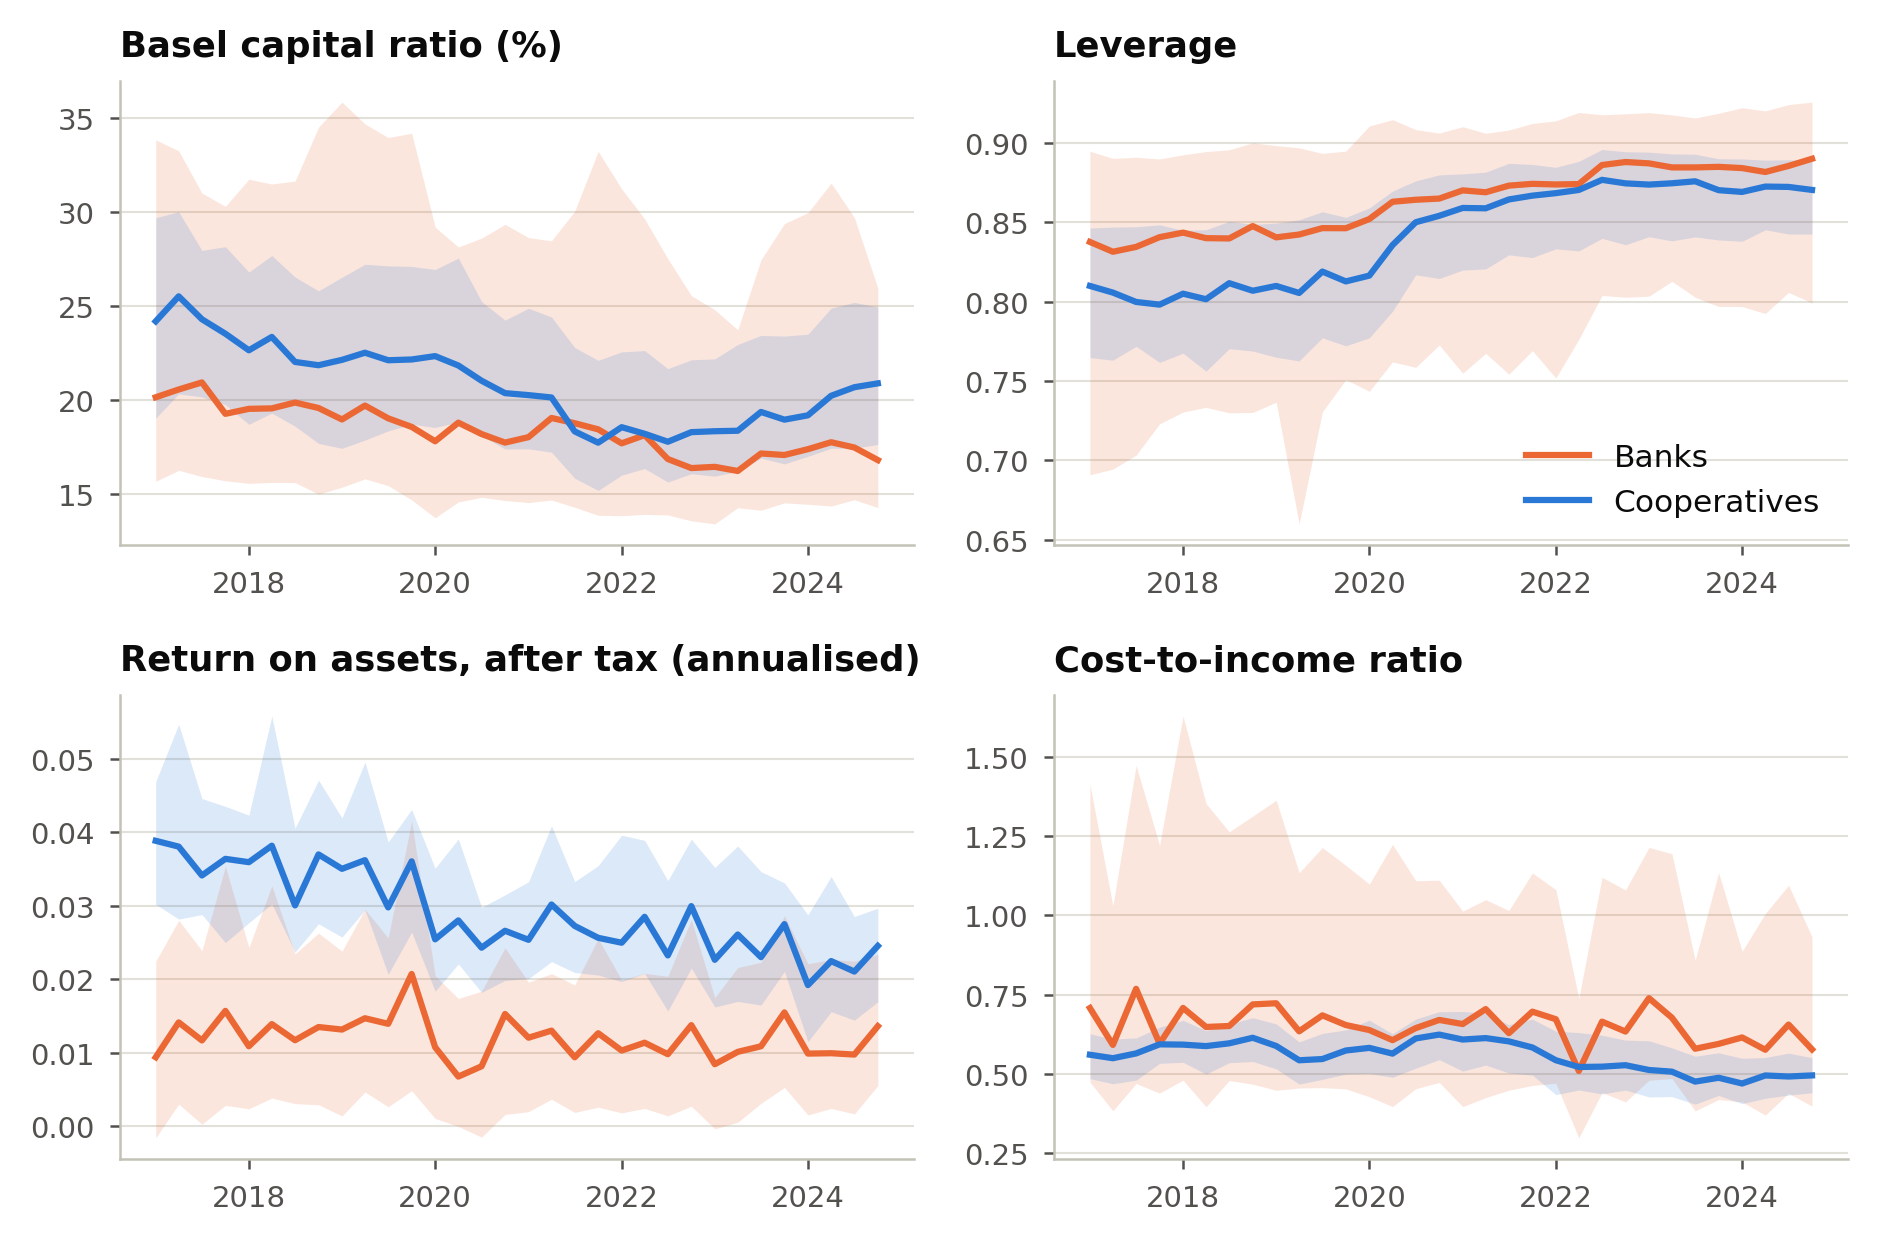
\includegraphics[width=\linewidth]{fig11_stable}
\column{0.3\textwidth}
\vspace{0.3cm}
\bignum{0.31}{residual s.d. of the capital ratio, cooperatives over banks, at equal size}\vspace{0.3cm}
\bignum{0.10}{same ratio for cost-to-income}\vspace{0.3cm}
{\footnotesize Lines are group medians, bands the interquartile range. The median cooperative is better capitalised than the median bank for most of the window. Dispersion ratios from tables/t8.}
\end{columns}
\note{One minute. The time series make the dispersion point visible. The blue bands are narrow on every outcome; the orange bands are wide. At equal size, the residual standard deviation among cooperatives is between a tenth and a half of the bank figure. Several differences that look large at the mean are differences in dispersion.}
\end{frame}

\begin{frame}{Profitability: the operating return and the tax wedge}
\begin{columns}[T]
\column{0.62\textwidth}
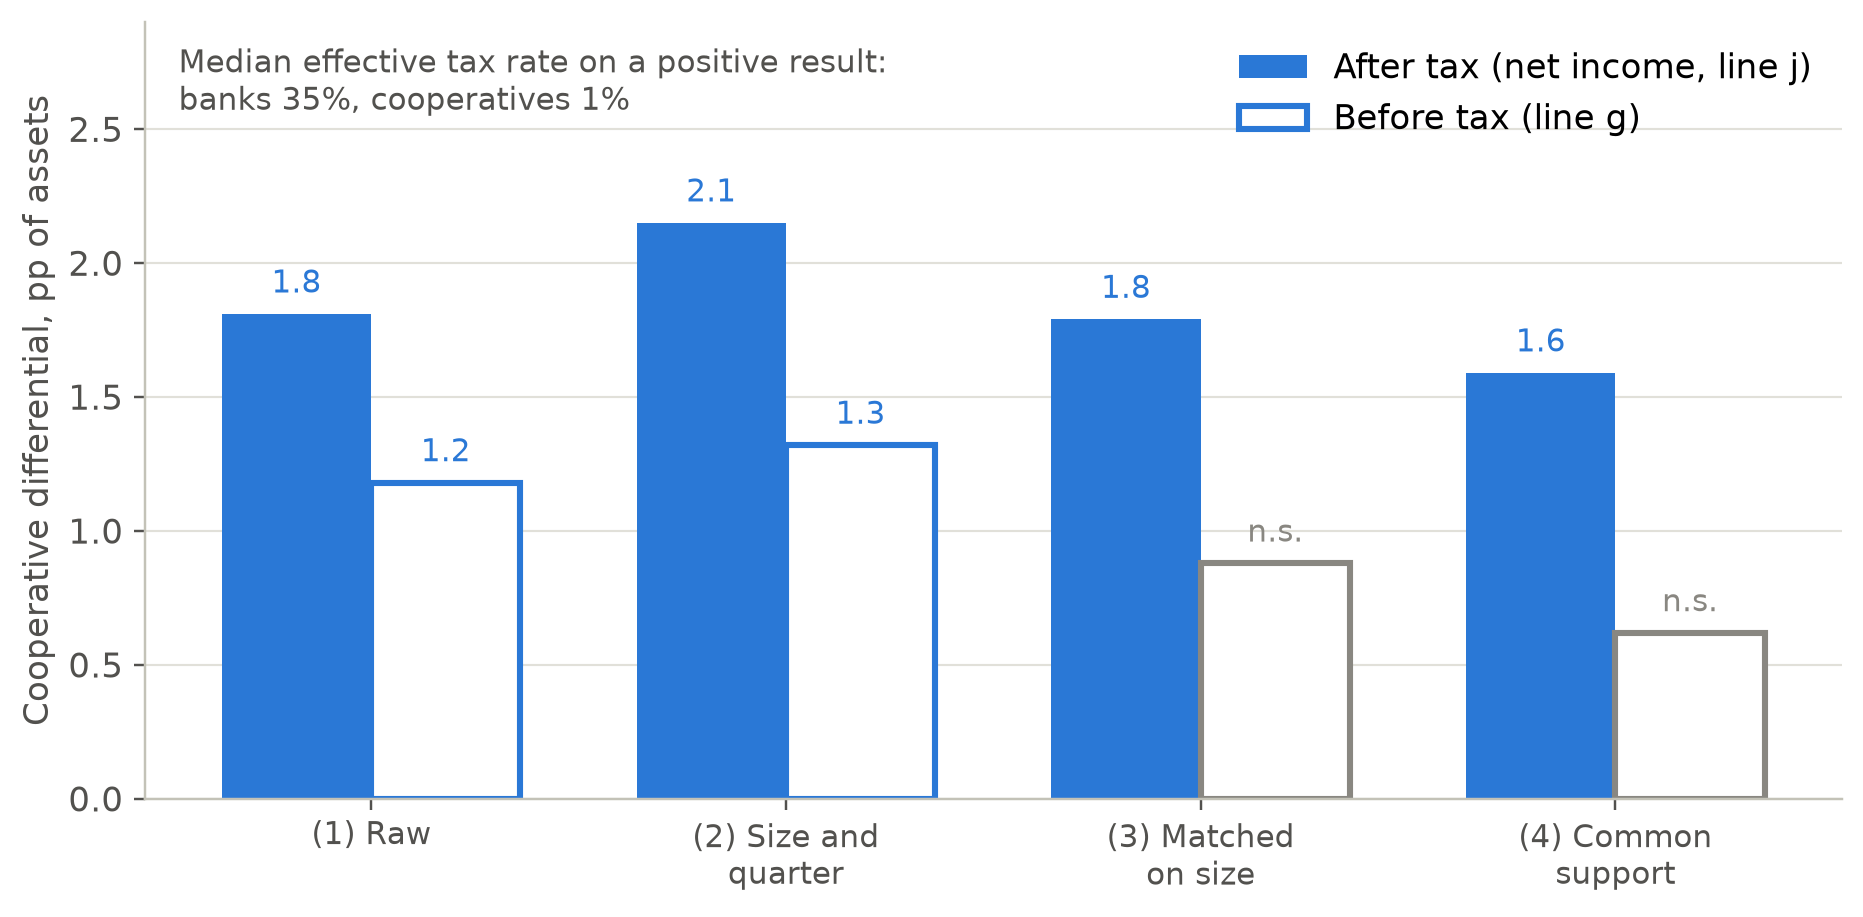
\includegraphics[width=\linewidth]{tax_wedge}
\column{0.36\textwidth}
\vspace{0.2cm}
\card{4.7cm}{After tax: stable}{About two percentage points of assets more than comparable banks, in every specification: the return a cooperative retains as capital.}
\card{4.7cm}{Before tax: null at the mean}{Positive at the median (1.4 pp, interval excludes zero; tables/t7). A high-earning bank tail pulls the mean towards zero.}
\card{4.7cm}{The wedge}{The pre-tax gap under controls is three fifths of the after-tax gap, so the tax exemption accounts for about two fifths.}
\end{columns}
\note{One minute. The typical cooperative earns more than a comparable bank before tax, but the mean gap is not established. After tax the gap is stable, and the distance between the two rows is the tax exemption of cooperative acts: median effective rate about a third for banks, close to zero for cooperatives. Cross-country evidence reports cooperatives as less profitable; here the disagreement is narrower than the after-tax figures suggest.}
\end{frame}

\begin{frame}{Capital: a modest gap in level, a large gap in dispersion}
\centerline{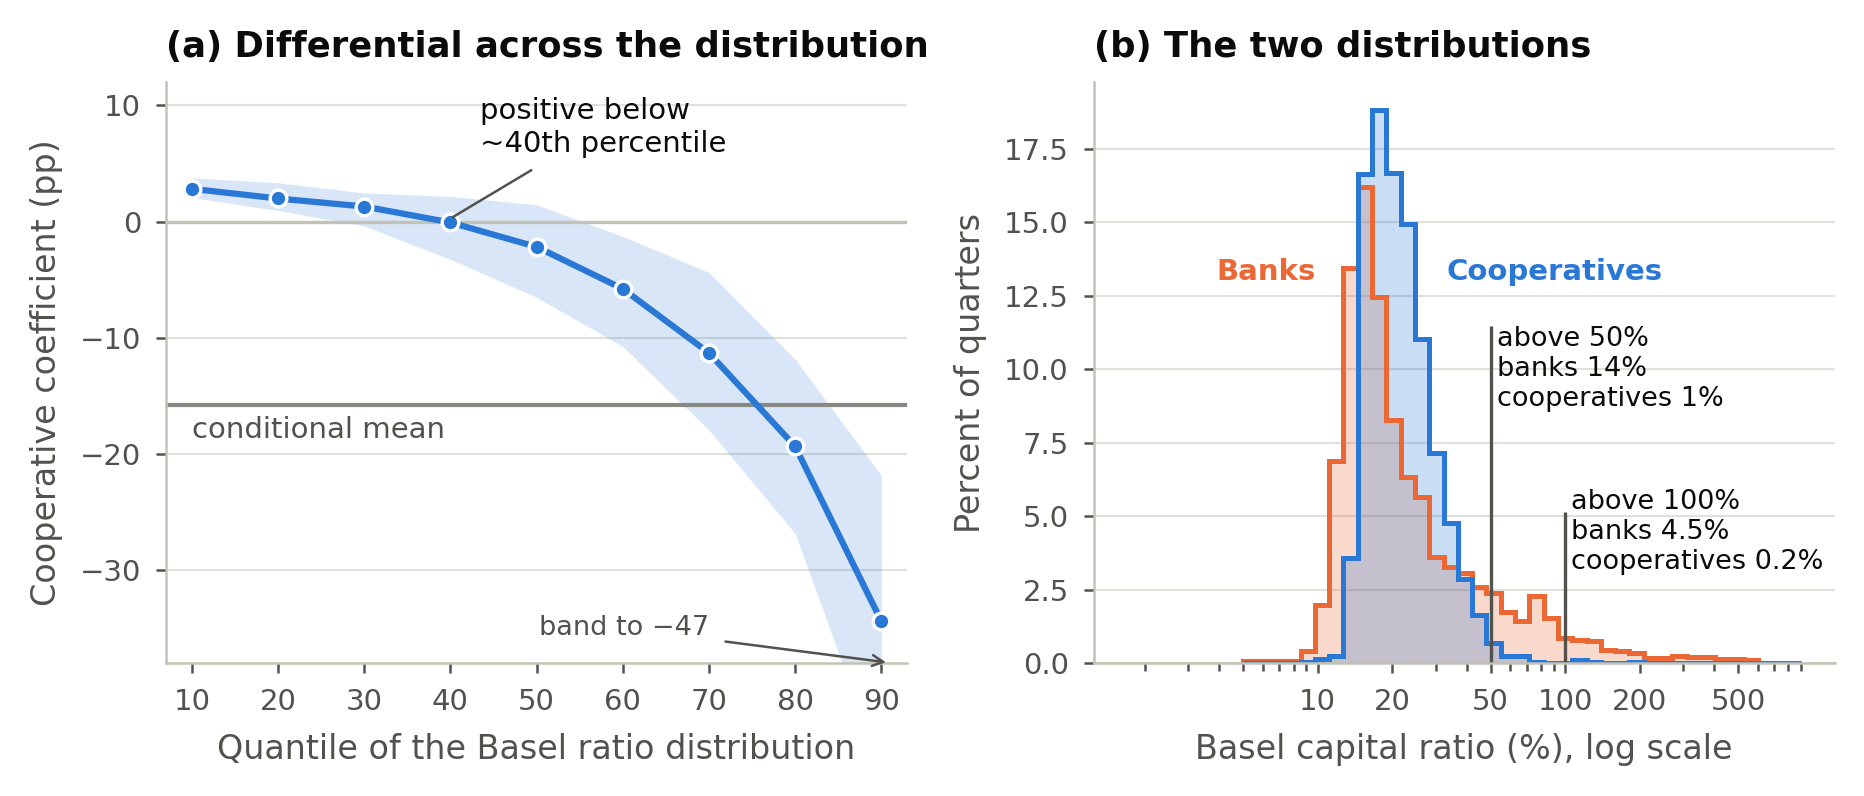
\includegraphics[width=0.58\linewidth]{fig12_capital_quantiles}}
\vspace{0.05cm}
\begin{columns}[T]
\column{0.32\textwidth}\bignum{$-$15.8 pp}{size-controlled mean gap; conditional median $-$2.2 pp}
\column{0.32\textwidth}\bignum{14\% vs 1\%}{bank and cooperative quarters above a Basel ratio of 50 percent}
\column{0.32\textwidth}\bignum{40th}{percentile where the coefficient crosses zero: positive below, negative above}
\end{columns}
\note{One and a half minutes. The capital result needs the most care. The mean gap is large and negative, but it is a statement about the bank upper tail: small standalone banks that barely intermediate and hold capital ratios above fifty, sometimes above one hundred percent. At the thin end of the distribution, where supervisors look, cooperatives hold more capital than banks at the same quantile, and they provision no less. Against deposit-funded banks the mean gap roughly halves. Leverage mirrors capital and is treated as one result with it.}
\end{frame}

\begin{frame}{Two often-cited differences vanish against banks}
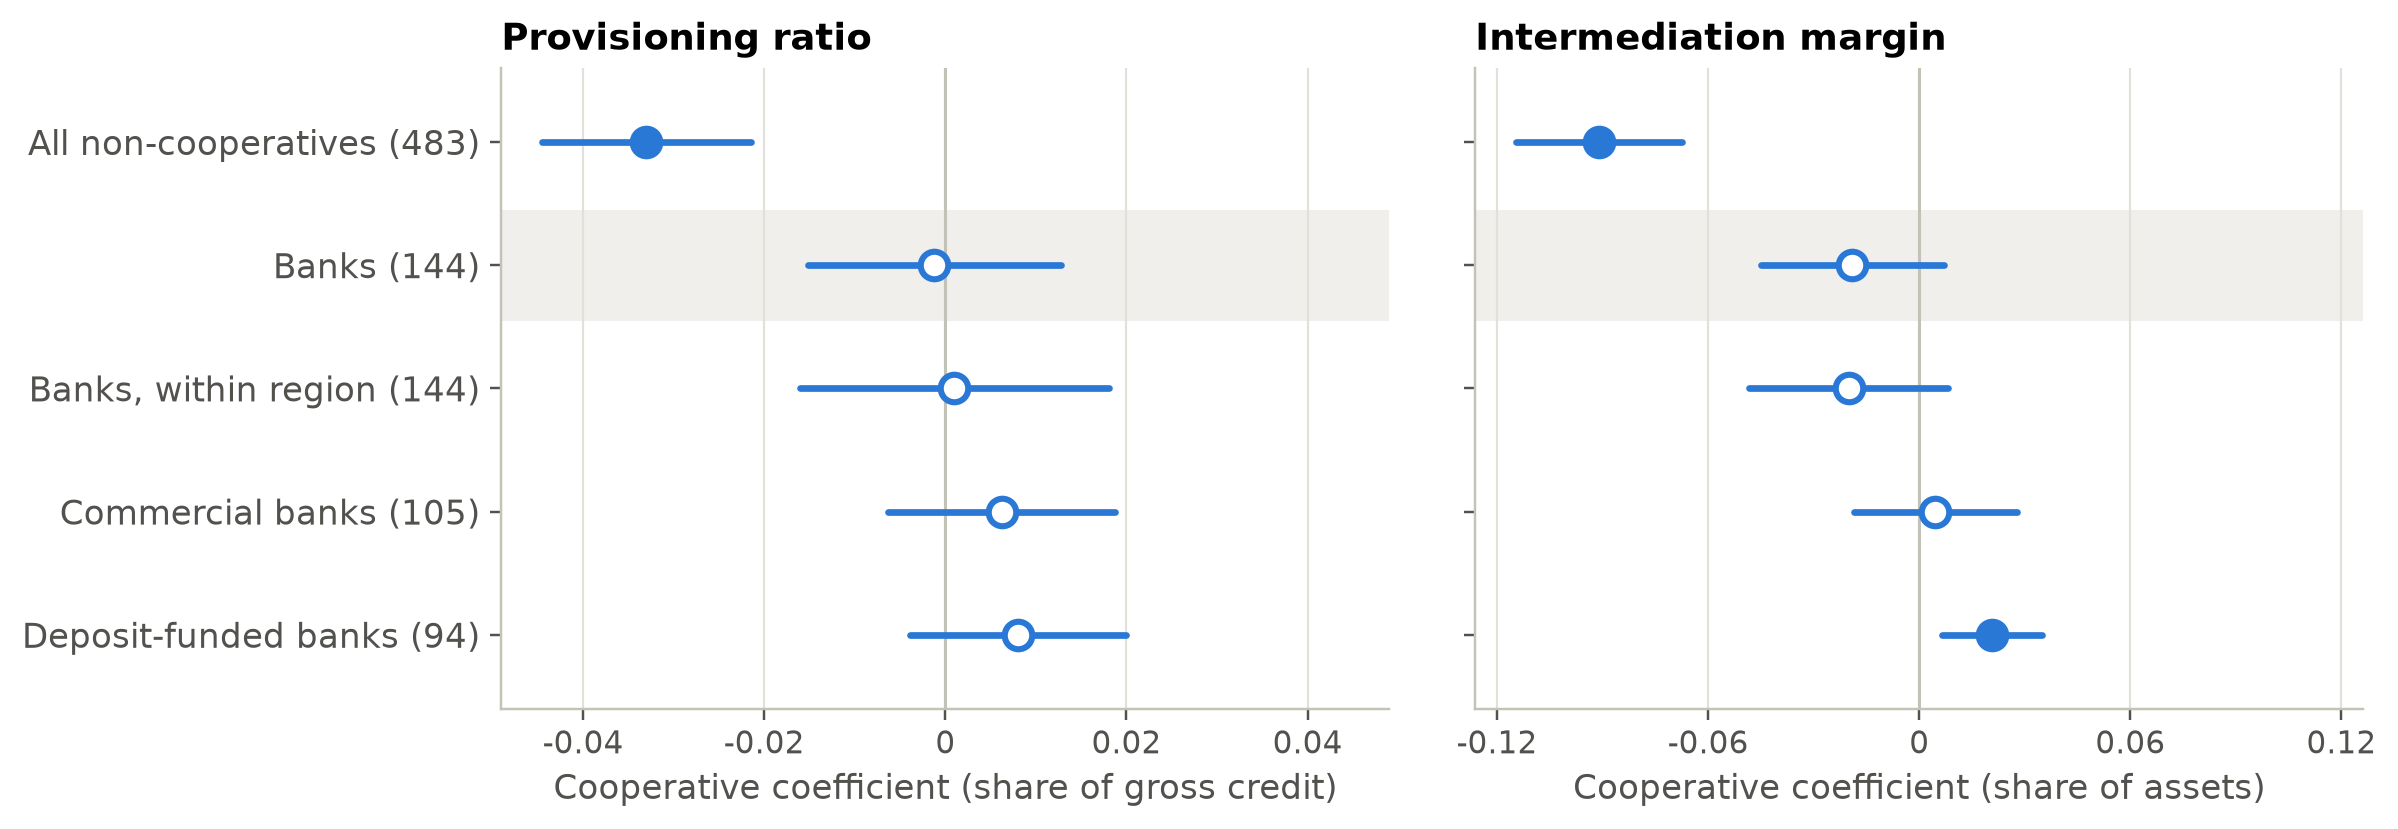
\includegraphics[width=\linewidth]{ladder_vanish}\par
\vspace{0.15cm}
{\centering\small Against all non-cooperatives, cooperatives appear to provision less and earn thinner margins. Against banks both coefficients sit at zero. The broad group holds 158 institutions with no credit and no funds raised, and non-banking lenders whose provisioning ratios are nearly three times those of banks and cooperatives.\par}
\note{One minute. Two claims the same data appear to support under a loose comparison group. Lower provisioning: significant at one percent against all non-cooperatives, zero against banks, and at the conditional median cooperatives provision more. Thinner margins: same pattern, and positive against deposit-funded banks. Neither survives. The comparison group is a result in itself.}
\end{frame}

\begin{frame}{What survives against which comparison group}
\begin{columns}[T]
\column{0.64\textwidth}
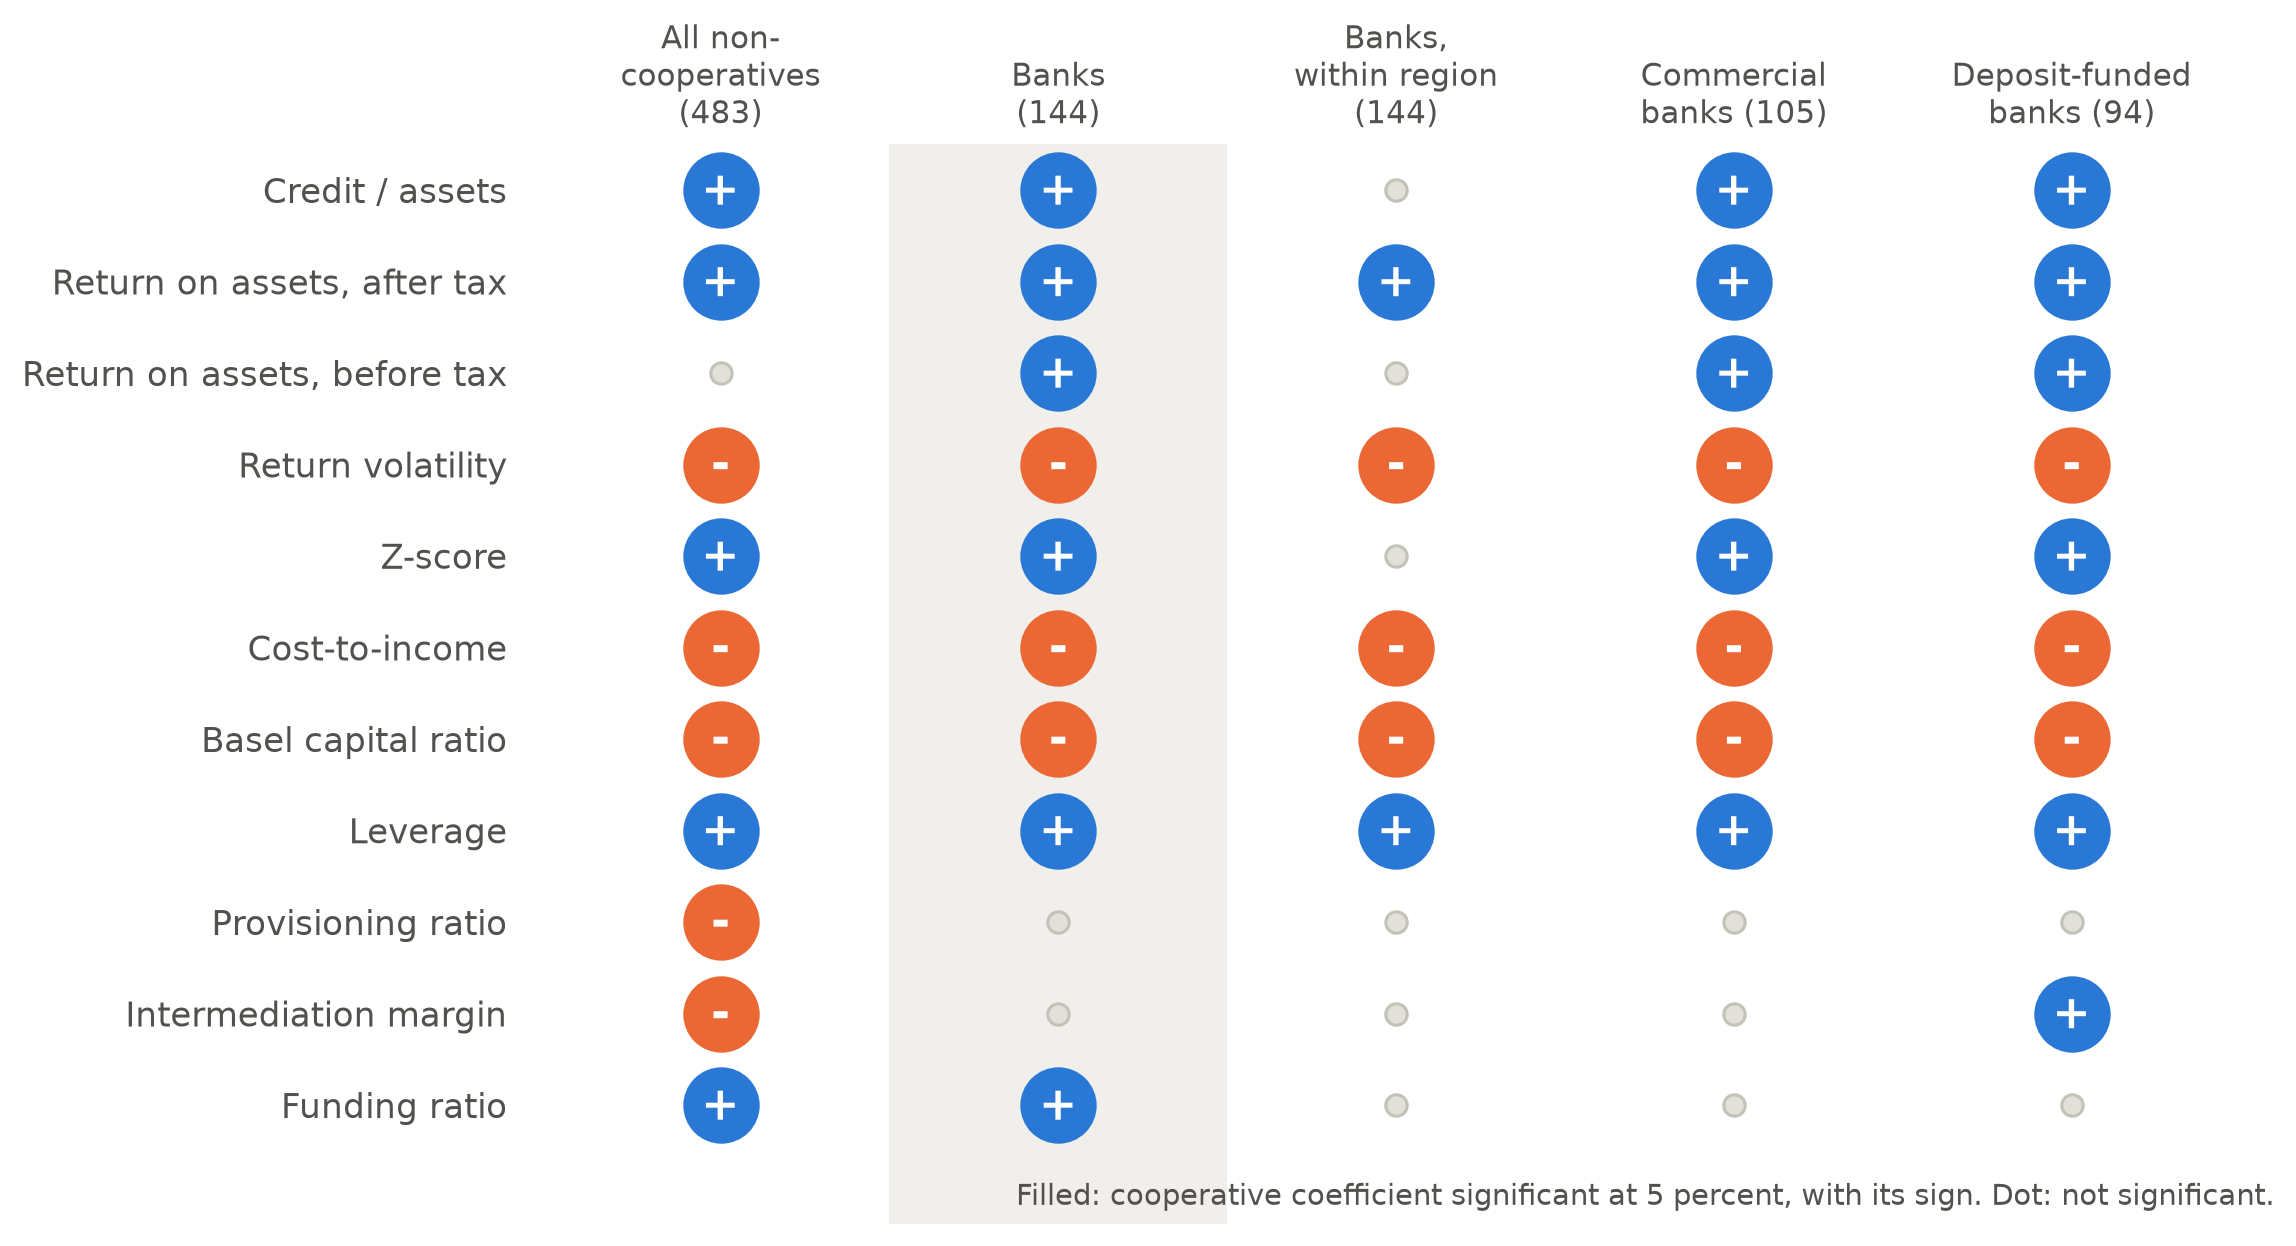
\includegraphics[width=\linewidth]{survival}
\column{0.34\textwidth}
\vspace{0.1cm}
\card{4.3cm}{Holds on every rung}{After-tax return, cost-to-income, return volatility, capital and leverage.}
\card{4.3cm}{Holds nationally, open within region}{Credit intensity: nearly a fifth of assets more than banks of the same size; zero within macro-region (effective control sample of about eighteen banks).}
\card{4.3cm}{Only against the broad group}{Lower provisioning and thinner margins.}
\end{columns}
\note{One minute. The survival matrix. Cost, return stability and the retained return hold against every definition of a bank we tried. Credit intensity holds nationally and is unshown within regional markets: whether region is a mediator or a confounder is an assumption the data cannot test, so we report both. Provisioning and margins appear only against the broad group.}
\end{frame}

\begin{frame}{What it means}
\vspace{0.2cm}
\begin{columns}[T]
\column{0.32\textwidth}\card{3.9cm}{For proportionality}{A benchmark calibrated on the average institution describes the lending cooperative poorly, since cooperatives do not inhabit the upper region of that distribution. Two margins beyond size: integrated networks and their backstops, and the calibration itself. Lighter requirements do not follow automatically.}
\column{0.32\textwidth}\card{3.9cm}{For the tax debate}{The exemption of cooperative acts appears in the retained return, the only capital a cooperative can build, and accounts for about two fifths of the after-tax differential. At the banks' effective rate, cooperative capital would grow about three tenths more slowly.}
\column{0.32\textwidth}\card{3.9cm}{For the movement}{Cost at the median and return stability hold against every definition of a bank. Profitability holds for the retained return and, before tax, at the median. More conservative provisioning does not hold. The territorial claim remains open.}
\end{columns}
\vspace{0.25cm}
{\centering\scriptsize\color{muted} Three analyst choices decided whether headline results existed: the comparison group, reading cumulative income fields as quarterly flows, and the matched estimand. Code and pipeline are public.\par}
\note{One minute. Three implications. For supervisors, the whole distribution matters as much as the mean, and the average institution is a poor benchmark for a focused retail lender. For the tax debate, we locate the exemption's effect without settling whether it is a subsidy or the recognition of mutual self-help. For the movement, which claims the data support and which they do not. Thank you; supplementary slides follow.}
\end{frame}

% ================================================================ backup
\divider{Supplementary}{Methods and details}{For questions}{Backup slides for questions.}

\begin{frame}{Supplementary: who is in the sample}
\begin{columns}[T]
\column{0.56\textwidth}
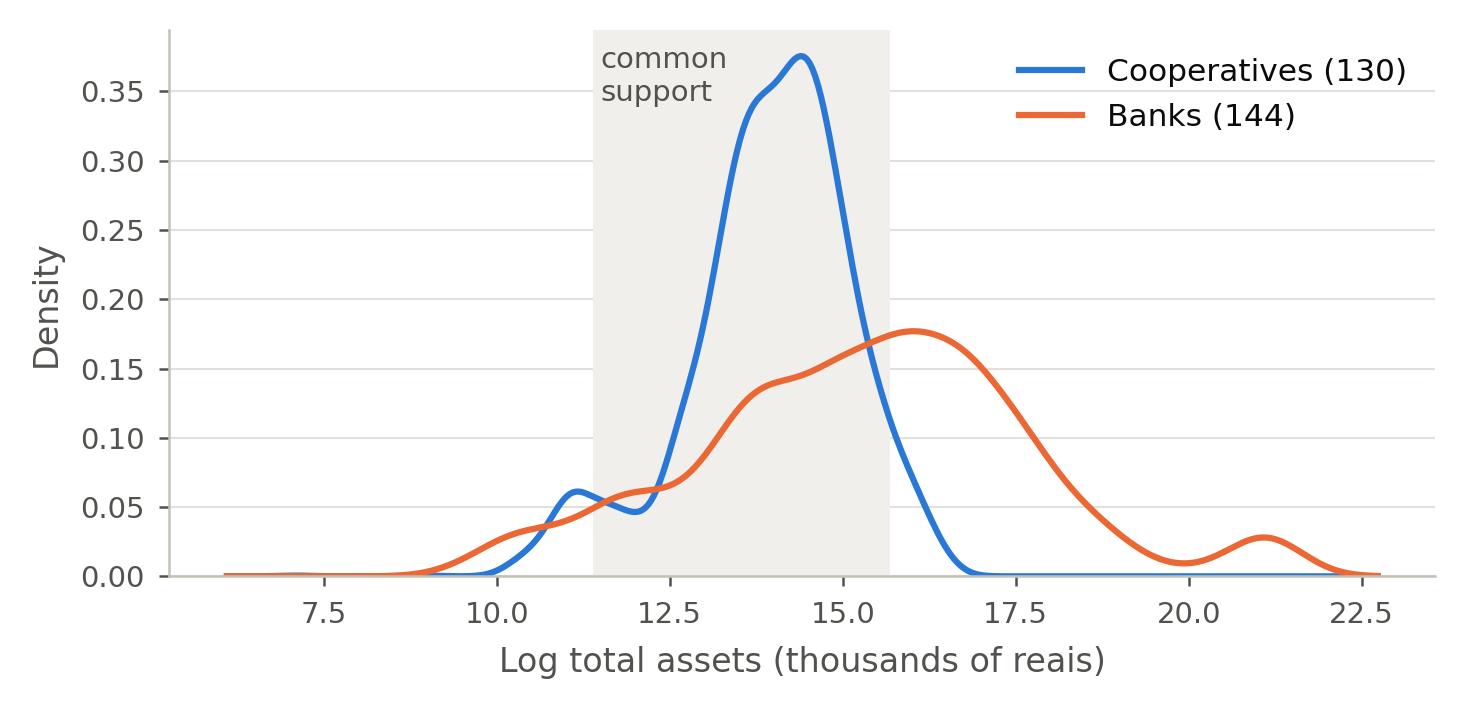
\includegraphics[width=\linewidth]{fig8_overlap}
\column{0.42\textwidth}
\vspace{0.1cm}
\card{5.4cm}{Common support}{Ninety percent of cooperative observations fall inside the common support in log assets, against 48 percent of bank observations. Matching and trimming bring the standardised difference from $-0.72$ to about zero.}
\card{5.4cm}{Classification}{On the Central Bank's consolidation type: b3S singular cooperative, b3C central (excluded). Each institution takes its modal type, so status is time-invariant; classification by name would place the sector's own banks on the cooperative side.}
\end{columns}
\note{The size distributions overlap in the middle; the largest banks have no cooperative counterpart and leave the matched sample.}
\end{frame}

\begin{frame}{Supplementary: who is in the broad comparison group}
\begin{columns}[T]
\column{0.56\textwidth}
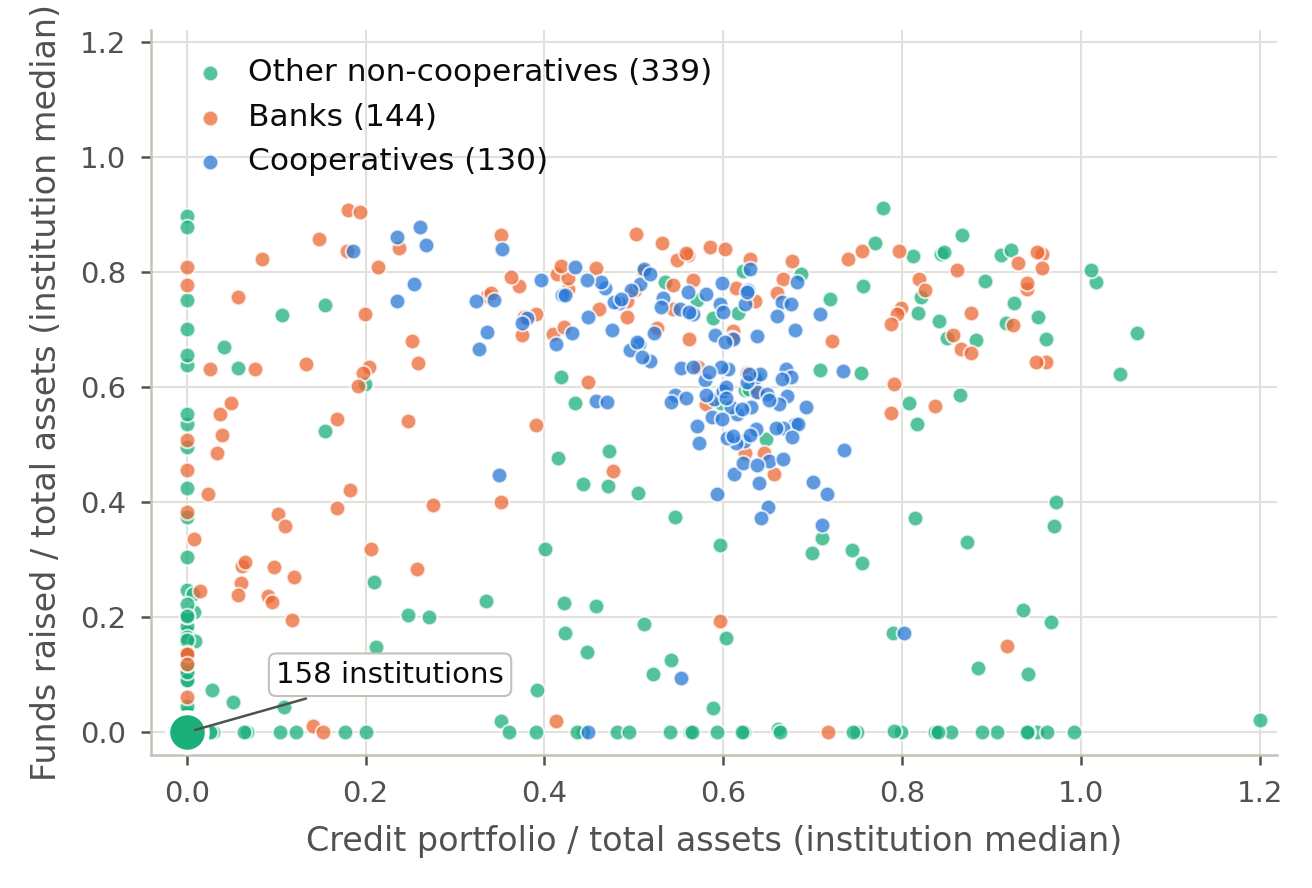
\includegraphics[width=\linewidth]{fig14_broad_group}
\column{0.42\textwidth}
\vspace{0.1cm}
\card{5.4cm}{339 institutions outside the bank rung}{Of these, 158 have a median of zero credit and zero funds raised, which makes the credit and funding differentials mechanical; the provisioning gap comes from non-banking lenders.}
\card{5.4cm}{No rung defined on lending}{Selecting peers on an outcome would build the credit result in. The broad group is reported because its divergence from banks is itself a result.}
\end{columns}
\note{Institution medians over 2017 to 2024. The cluster of cooperatives sits where banks sit; the broad group spreads along both axes.}
\end{frame}

\begin{frame}{Supplementary: two measurement corrections}
\begin{columns}[T]
\column{0.48\textwidth}
\card{6.0cm}{Income fields accumulate within the semester}{Brazilian institutions close balance sheets in June and December, and IF.data income fields reset at each date. Flows are de-cumulated and annualised, which scales the return coefficient by about 2.7 relative to reading the cumulative field as a quarterly rate; the de-cumulated medians match the Central Bank's published figures.}
\column{0.48\textwidth}
\card{6.0cm}{The intermediation result is net of provisions}{The expense subtotal contains the loan-loss provision line, so the reported result partly reproduces the provisioning outcome under another name. The margin is computed gross of provisions, and the cost-to-income denominator likewise.}
\card{6.0cm}{Provisioning is an accounting variable}{Stock of provisions under Resolution 2.682/1999 over gross credit; minimum provisions follow the AA to H rating grid, independent of ownership. A weak proxy for realised delinquency.}
\end{columns}
\note{Both corrections changed at least one conclusion in the original notebook.}
\end{frame}

\begin{frame}{Supplementary: the cooperative differential against banks}
\scriptsize
\begin{center}
\footnotesize
\setlength{\tabcolsep}{3pt}
\begin{tabular}{lrrrrrrl}
\toprule
Outcome & (1) Raw & (2) Controls & (3) CEM & (4) Trim & Median (2) & $\rho$ & Tier \\
\midrule
Basel capital ratio (pp) & -8.19$^{***}$ & -15.77$^{***}$ & -17.50$^{***}$ & -14.21$^{***}$ & -2.18 & 1.73 & stable in sign \\
Leverage & 0.0561$^{**}$ & 0.1220$^{***}$ & 0.1046$^{***}$ & 0.0813$^{***}$ & 0.0283 & 1.45 & stable in sign \\
Return on assets, after tax & 0.0181$^{***}$ & 0.0215$^{***}$ & 0.0179$^{***}$ & 0.0159$^{***}$ & 0.0171 & 0.88 & stable \\
Return on assets, before tax & 0.0118$^{***}$ & 0.0132$^{**}$ & 0.0088 & 0.0062 & 0.0144 &  & null \\
Cost-to-income ratio & -0.6025$^{***}$ & -0.7923$^{***}$ & -0.8385$^{***}$ & -0.7522$^{***}$ & -0.1796 & 1.25 & stable in sign \\
Credit portfolio / assets & 0.1654$^{***}$ & 0.1881$^{***}$ & 0.1701$^{***}$ & 0.1780$^{***}$ & 0.2448 & 1.08 & stable \\
Provisioning ratio & 0.0020 & -0.0012 & 0.0010 & 0.0009 & 0.0236 &  & null \\
Intermediation margin & -0.0003 & -0.0190 & -0.0107 & -0.0171 & 0.0203 &  & null \\
Funding ratio & 0.0461 & 0.0887$^{**}$ & 0.0536 & 0.0330 & -0.0247 &  & null \\
\midrule
Return on assets volatility & -0.0110$^{***}$ & -0.0189$^{***}$ & -0.0175$^{***}$ & -0.0170$^{***}$ & -0.0133 & 1.55 & stable \\
Z-score & 4.20$^{***}$ & 6.32$^{***}$ & 6.14$^{***}$ & 6.20$^{***}$ & 7.58 & 1.48 & stable \\
\bottomrule
\end{tabular}
\begin{tablenotes}[flushleft]\footnotesize
\item Standard errors clustered by institution, HC3 for the last two rows; * p<0.05, ** p<0.01, *** p<0.001, confirmed by a wild cluster bootstrap. Median (2): conditional median of column (2). rho = |b\_trim|/|b\_raw|. Tier: see Section 3.4.
\end{tablenotes}

\end{center}
\note{The main table of the paper.}
\end{frame}

\begin{frame}{Supplementary: quantile regression coefficients}
\begin{center}
\scriptsize
\begin{threeparttable}
\footnotesize
\setlength{\tabcolsep}{2.5pt}
\begin{tabular}{lrrrrrr}
\toprule
Outcome & $q_{10}$ & $q_{25}$ & $q_{50}$ & $q_{75}$ & $q_{90}$ & Mean \\
\midrule
Basel ratio (pp) & 2.81 & 1.61 & -2.18 & -14.23 & -34.37 & -15.77 \\
 & [2.06, 3.75] & [0.19, 2.76] & [-6.52, 1.43] & [-22.45, -8.20] & [-47.28, -21.82] & [-21.93, -9.62] \\
Leverage & 0.294 & 0.117 & 0.028 & -0.009 & -0.023 & 0.122 \\
 & [0.194, 0.370] & [0.069, 0.174] & [0.003, 0.062] & [-0.021, 0.008] & [-0.037, -0.007] & [0.082, 0.162] \\
Return on assets, after tax & 0.044 & 0.026 & 0.017 & 0.010 & -0.006 & 0.021 \\
 & [0.032, 0.062] & [0.020, 0.030] & [0.014, 0.021] & [0.005, 0.015] & [-0.017, 0.004] & [0.014, 0.029] \\
Return on assets, before tax & 0.052 & 0.028 & 0.014 & -0.003 & -0.029 & 0.013 \\
 & [0.038, 0.066] & [0.023, 0.035] & [0.009, 0.019] & [-0.011, 0.005] & [-0.046, -0.016] & [0.004, 0.023] \\
Cost-to-income & 0.110 & 0.006 & -0.180 & -0.647 & -1.756 & -0.792 \\
 & [0.009, 0.151] & [-0.051, 0.067] & [-0.277, -0.107] & [-0.870, -0.438] & [-2.822, -1.158] & [-1.047, -0.538] \\
Credit / assets & 0.383 & 0.424 & 0.245 & -0.019 & -0.170 & 0.188 \\
 & [0.343, 0.428] & [0.370, 0.466] & [0.146, 0.363] & [-0.085, 0.069] & [-0.219, -0.111] & [0.129, 0.248] \\
Provisioning ratio & 0.030 & 0.030 & 0.024 & 0.001 & -0.054 & -0.001 \\
 & [0.026, 0.033] & [0.026, 0.034] & [0.018, 0.029] & [-0.016, 0.015] & [-0.093, -0.017] & [-0.015, 0.013] \\
\bottomrule
\end{tabular}
\begin{tablenotes}[flushleft]\footnotesize
\item Quantile regressions on the cooperative dummy, log assets and quarter effects; the last column is OLS. Brackets: 95 percent institution-bootstrap intervals (199 draws) and the clustered interval for the mean.
\end{tablenotes}

\end{threeparttable}
\end{center}
\note{Quantile regressions on the cooperative dummy, log assets and quarter effects; the last column is OLS. Capital, leverage and cost-to-income change sign across the distribution; the pre-tax return is positive up to the median and negative in the top decile.}
\end{frame}

\begin{frame}{Supplementary: dispersion at equal size}
\begin{columns}[T]
\column{0.56\textwidth}
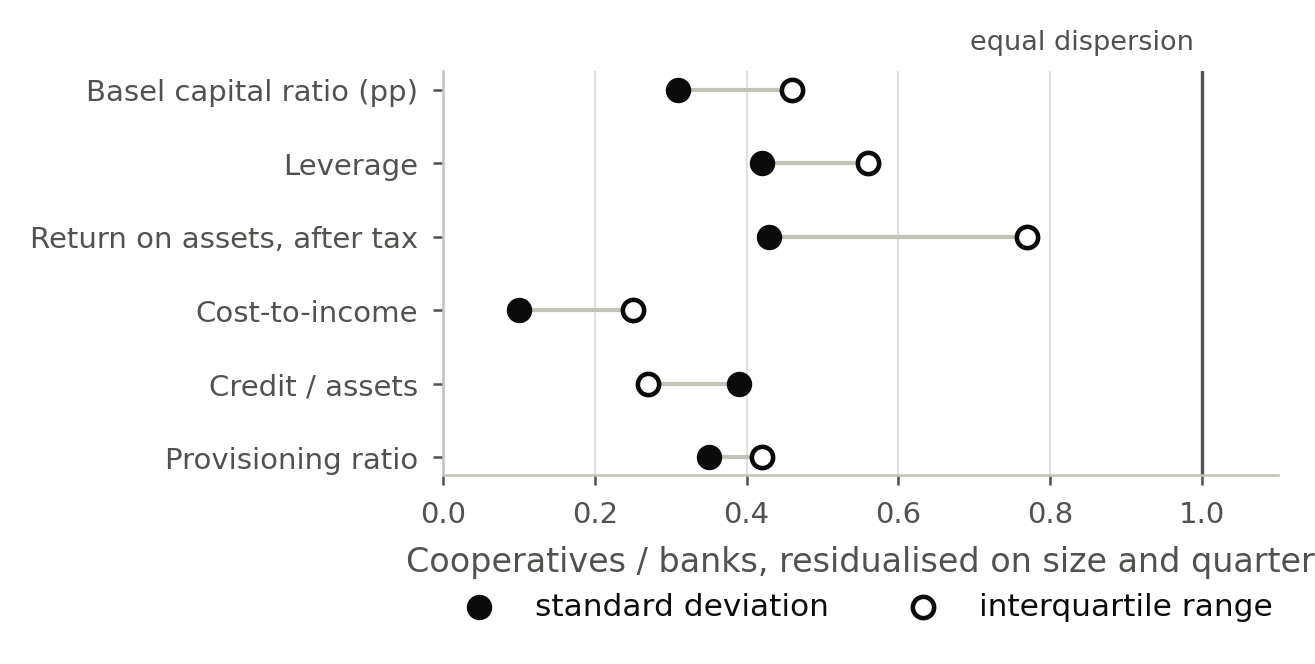
\includegraphics[width=\linewidth]{fig16_dispersion}
\column{0.42\textwidth}
\vspace{0.1cm}
\card{5.4cm}{Residuals from log assets and quarter effects}{Cooperative over bank residual s.d.: capital 0.31, leverage 0.42, after-tax return 0.43, cost-to-income 0.10, credit 0.39, provisioning 0.35 (tables/t8); generalised variance ratio over seven outcomes 0.08.}
\card{5.4cm}{Reading}{Cooperatives are the more homogeneous group on every outcome. Endowment capital predicts a narrow band: no reason to hold capital far above what lending requires, and no outside investor to supply it.}
\end{columns}
\note{The dispersion result underlies the reading of the capital gap.}
\end{frame}

\begin{frame}{Supplementary: the bank upper tail sits among banks reporting individually}
\small
\begin{center}
\begin{tabular}{lrrrrrr}
\toprule
Group & Institutions & Quarters & Mean & Median & $p_{90}$ & Share $>50\%$ \\
\midrule
Banks, conglomerate consolidations & 87 & 2,604 & 22.7 & 16.8 & 39.2 & 6.4 \\
Banks, individual & 57 & 1,580 & 44.5 & 24.5 & 109.1 & 26.4 \\
Cooperatives (all individual) & 130 & 3,050 & 22.8 & 20.5 & 32.9 & 1.0 \\
\bottomrule
\end{tabular}
\end{center}
{\footnotesize Basel ratio, winsorised analysis sample (tables/t11, panel A). Against individually reporting banks the controlled capital gap is $-21.4$ pp; against prudential conglomerates, $-5.4$ pp. Against deposit-funded banks the share of bank-quarters above 50 percent falls to 7.5 percent and the mean gap roughly halves while remaining significant.}
\note{Two features locate the tail: it sits among banks that report individually, and it thins when banks must be deposit-funded in every quarter.}
\end{frame}

\begin{frame}{Supplementary: heterogeneity by cooperative system}
\begin{center}
\scriptsize
\begin{threeparttable}
\begin{tabular}{lrrrrrr}
\toprule
System & Inst. & Treated & Basel (pp) & Leverage & ROA & Provisioning \\
\midrule
Sicredi & 106 & 106 & -17.35$^{***}$ & 0.1341$^{***}$ & 0.0219$^{***}$ & -0.0008 \\
Sicoob & 17 & 17 & -10.98$^{*}$ & 0.0847$^{*}$ & 0.0164$^{*}$ & -0.0007 \\
Independent & 6 & 5 & 6.90 & -0.0313 & 0.0287$^{*}$ & -0.0165 \\
Cresol & 1 & -- & \multicolumn{4}{c}{fewer than five institutions, not estimated} \\
\bottomrule
\end{tabular}
\begin{tablenotes}[flushleft]\footnotesize
\item Controlled specification against the bank group. Stars from the restricted wild cluster bootstrap: * p<0.05, ** p<0.01, *** p<0.001. Treated: cooperative clusters with a usable observation; with five, the smallest attainable bootstrap p-value is about 0.03. Sicoob's capital coefficient has a bootstrap p-value of 0.019. The independent return-on-assets coefficient has an asymptotic p-value below 0.001 and a bootstrap p-value of 0.033.
\end{tablenotes}

\end{threeparttable}
\end{center}
\note{Sicredi and Sicoob account for all but seven cooperatives. Both hold less regulatory capital than comparable banks; the six independents point the other way and are too few to measure. A network backstop is one candidate explanation, entangled with size, geography, business mix and governance. Provisioning is insignificant in every system.}
\end{frame}

\begin{frame}{Supplementary: before and after the 2022 capital rules}
\begin{center}
\footnotesize
\begin{threeparttable}
\begin{tabular}{lrrr}
\toprule
Outcome & Full sample & 2017Q1--2021Q4 & 2022Q1--2024Q4 \\
\midrule
Basel capital ratio (pp) & -15.77$^{***}$ & -16.90$^{***}$ & -13.96$^{***}$ \\
Leverage & 0.1220$^{***}$ & 0.1337$^{***}$ & 0.1033$^{***}$ \\
Return on assets, after tax & 0.0215$^{***}$ & 0.0242$^{***}$ & 0.0173$^{***}$ \\
Return on assets, before tax & 0.0132$^{**}$ & 0.0145$^{*}$ & 0.0111$^{*}$ \\
Cost-to-income ratio & -0.7923$^{***}$ & -0.8533$^{***}$ & -0.6927$^{***}$ \\
Credit portfolio / assets & 0.1881$^{***}$ & 0.2046$^{***}$ & 0.1629$^{***}$ \\
Provisioning ratio & -0.0012 & -0.0082 & 0.0104 \\
Intermediation margin & -0.0190 & -0.0251 & -0.0093 \\
Funding ratio & 0.0887$^{**}$ & 0.1128$^{***}$ & 0.0508 \\
\midrule
Observations & 7,234 & 4,436 & 2,798 \\
Cooperatives & 130 & 112 & 120 \\
Banks & 144 & 141 & 134 \\
\bottomrule
\end{tabular}
\begin{tablenotes}[flushleft]\footnotesize
\item Controlled specification, cooperatives against banks, on the full sample and on each subperiod; the boundary is 3 January 2022, when Resolutions CMN 4.955 and 4.958 took effect. Standard errors clustered by institution. Bootstrap p-values (1,999 replications) agree with the clustered stars in every cell.
\end{tablenotes}

\end{threeparttable}
\end{center}
\note{Every surviving result keeps its sign and significance in both subperiods; magnitudes are roughly a fifth smaller after 2022. Excluding the eleven S1 and S2 banks moves no significant coefficient by more than two percent.}
\end{frame}

\begin{frame}{Supplementary: the ladder, outcome by outcome}
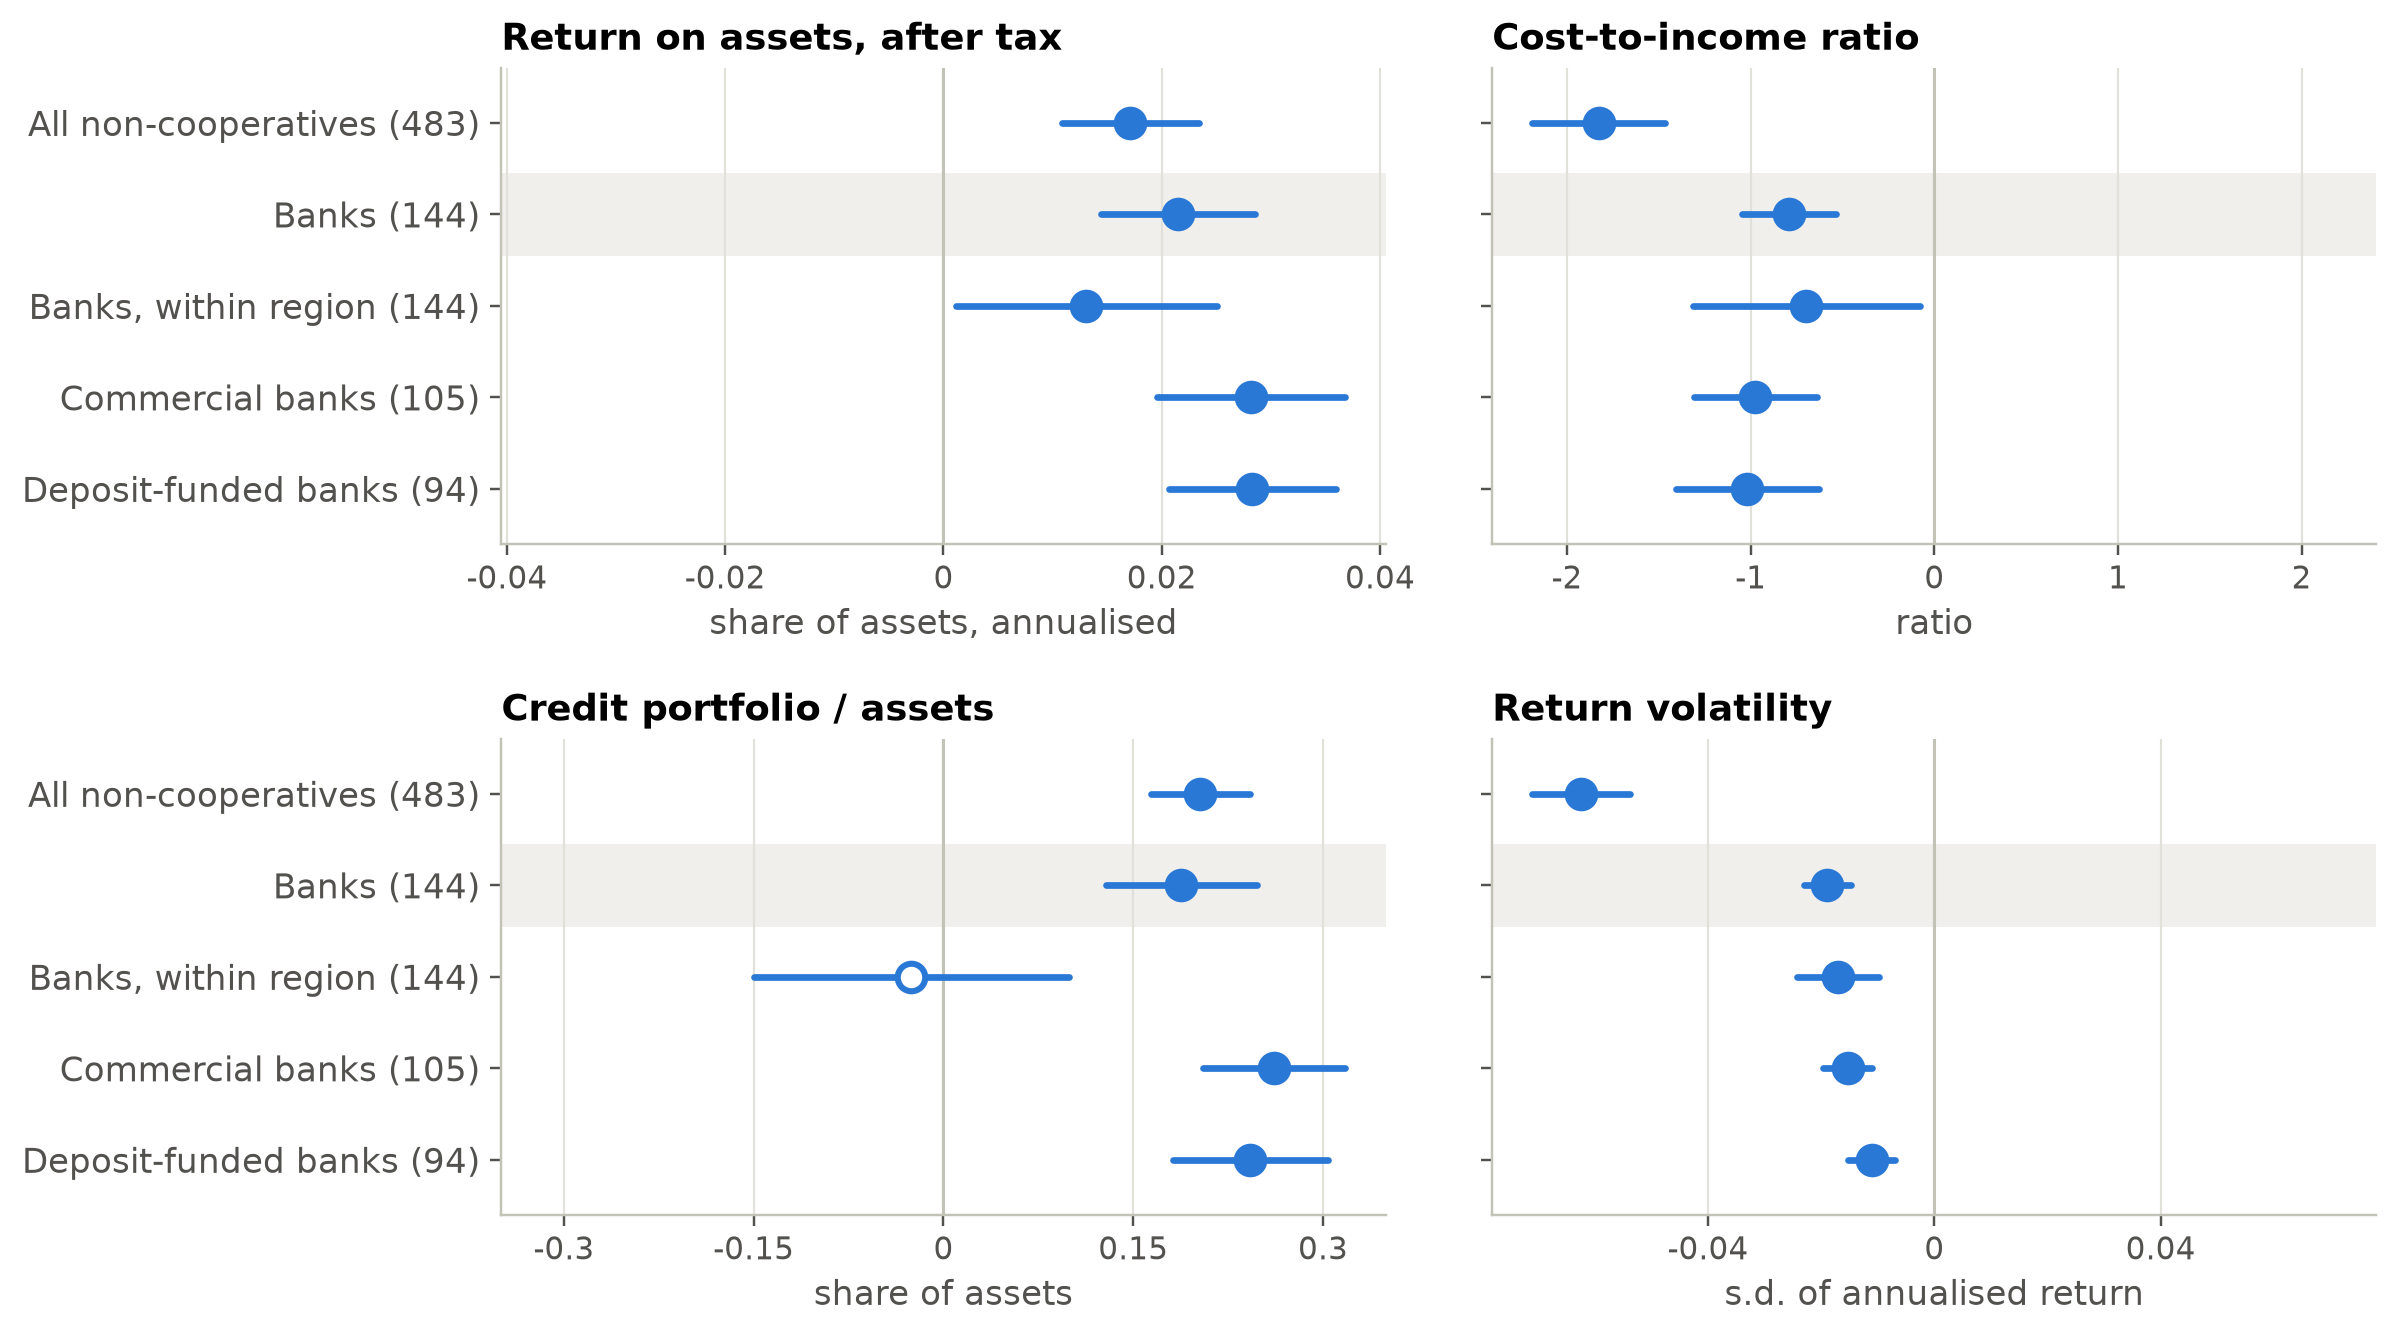
\includegraphics[width=0.92\linewidth]{ladder_survive}
\note{Controlled specification; within region uses the matched specification. Filled markers are significant at five percent.}
\end{frame}

\begin{frame}{Supplementary: credit intensity within and across regional markets}
\begin{columns}[T]
\column{0.48\textwidth}
\card{6.0cm}{Nationally}{Matched on size alone, cooperatives allocate nearly a fifth of assets more to credit than comparable banks, significant at one percent in every specification; at the conditional median, about a quarter.}
\card{6.0cm}{Within macro-region}{Matched also on region, the differential is small and indistinguishable from zero under any coarsening scheme. Cooperatives concentrate in the South, banks in the Southeast; the effective control sample is about eighteen banks.}
\column{0.48\textwidth}
\card{6.0cm}{Which estimate is the parameter}{If cooperatives concentrate where they do for reasons internal to member-based finance, region is a mediator and the national estimate is the parameter. If regional market structure is unrelated to form, region is a confounder and credit intensity is a null. The assumption is untestable here, so both are reported.}
\card{6.0cm}{Next step}{A market measure finer than macro-region, and IF.data's credit-modality modules, which carry rural credit.}
\end{columns}
\note{The territorial claim is the one these data leave open.}
\end{frame}

\begin{frame}{Supplementary: selection into the full methodology}
\begin{columns}[T]
\column{0.48\textwidth}
\card{6.0cm}{Who adopts}{The cooperatives observed are the largest in the country, about a tenth of all cooperatives in the panel. Fifty-one are observed under the simplified methodology before adopting the full one.}
\card{6.0cm}{Adopters against never-adopters, pre-adoption quarters}{No difference in leverage; adopters were less credit-intensive ($-0.068$, $p = 0.002$), marginally less profitable and marginally leaner.}
\column{0.48\textwidth}
\card{6.0cm}{What it means}{The estimates describe the adopters. The wider cooperative population would, if anything, show larger credit and profitability differentials and a smaller efficiency one.}
\card{6.0cm}{No regime effect}{A within-institution design around adoption fails to identify one: adoption follows growth, and pre-adoption trends run through the adoption date without a break.}
\end{columns}
\note{Selection bears on generalisation, not on the estimates.}
\end{frame}

\begin{frame}{Supplementary: literature and expectations}
\begin{columns}[T]
\column{0.48\textwidth}
\card{6.0cm}{Expected from theory}{Less regulatory capital in a narrower band (endowment capital, Fonteyne 2007; property-rights problems, Cook 1995); a higher share of assets in credit; lower return volatility (Hesse and \v{C}ih\'ak 2007). No sign committed on profitability and efficiency; no difference expected in provisioning or margin, which follow a regulatory grid.}
\column{0.48\textwidth}
\card{6.0cm}{Against the cross-country evidence}{Agreement on lower capitalisation at comparable size and lower return volatility. Disagreement on profitability: in this population the typical cooperative earns more before tax at the median, retains more after tax, and is less volatile on both measures. Part is the tax exemption; part may reflect a population of the largest cooperatives.}
\card{6.0cm}{Brazilian strand}{Bressan et al. 2011, Carvalho et al. 2015, Silva et al. 2023 (PEARLS on S4 credit unions, who proposed the comparison with banks of the same segment).}
\end{columns}
\note{Expectations were stated before the results; the study was not pre-registered.}
\end{frame}

\begin{frame}{Supplementary: limitations}
\begin{columns}[T]
\column{0.48\textwidth}
\card{6.0cm}{Identification}{Cooperative status is time-invariant, so the estimates are conditional correlations, not causal effects of form.}
\card{6.0cm}{Population}{The full-methodology restriction selects the largest cooperatives; results generalise to that subpopulation.}
\card{6.0cm}{Measures}{Provisioning is an accounting variable. Stability outcomes are institution-level statistics on a subsample with at least eight quarters.}
\column{0.48\textwidth}
\card{6.0cm}{Networks}{Most systems are too thin for separate inference. The backstop hypothesis needs consolidated network data that IF.data does not carry; centrals held about six percent of the singulars' regulatory capital at end-2024, so consolidation would move the differentials by far less than their size.}
\card{6.0cm}{Markets}{The mediator question needs a market measure finer than macro-region.}
\end{columns}
\note{The main limitations, for questions.}
\end{frame}

\end{document}
